\subsection{Phân tích đối thủ cạnh tranh}

Thị trường công cụ hỗ trợ livestream bán hàng tại Việt Nam đã có nhiều giải pháp,
cho thấy nhu cầu là có thật; tuy nhiên các giải pháp này phục vụ những bài toán
khác nhau và phần lớn chưa tập trung trọn vẹn vào phân khúc shop nhỏ/SME. Nhóm
phân tích đối thủ theo hai lớp:
\newline 
 \textbf{- Đối thủ trực tiếp} là các nền tảng cùng
phục vụ hoạt động livestream bán hàng, chia thành bốn nhóm: (i) AI livestream /
virtual host, (ii) phần mềm social commerce / chốt đơn, (iii) công cụ phát
livestream từ video có sẵn, và (iv) chatbot bán hàng đa kênh. 
\newline
\textbf{- Đối thủ gián tiếp} là quy trình thủ công hiện tại của người bán --- tự trực bình luận và
tra cứu sản phẩm từ Excel/Google Sheet/Zalo. Mỗi đối thủ được đánh giá theo ba
khía cạnh: năng lực nổi bật, giới hạn đối với shop nhỏ/SME, và khoảng trống mà
1Stream khai thác.

\subsubsection*{a. Nhóm AI livestream / virtual host: iLive, AnyLive}
\textbf{iLive (by SHOPNOW)} là hệ sinh thái A.I Social Selling gồm A.I Livestream,
A.I Video và A.I Digital Human, cung cấp hơn 100 avatar A.I, host ảo tùy chỉnh,
trình tạo kịch bản bằng A.I và livestream phát 24/7 trên Shopee/TikTok/Facebook;
mô hình tính phí theo giờ vận hành (khoảng 180.000--250.000đ/giờ, gói tối thiểu
180 giờ/tháng). \textbf{AnyLive (by AnyMind Group)} là nền tảng A.I Live Commerce
theo hướng tương tự, nhắm tới thương hiệu và doanh nghiệp có quy mô khu vực.
\newline
\textbf{- Giới hạn:} cả hai thiên về sản xuất hình ảnh host ảo và duy trì phát
sóng, công nghệ cao cấp nhưng có thể ``thừa'' và nặng chi phí với shop nhỏ chỉ
cần công cụ vận hành đơn giản; phản hồi bình luận chủ yếu theo kịch bản định sẵn,
chưa gắn chặt với dữ liệu sản phẩm riêng của từng shop.
\newline
 \textbf{- Khoảng trống:}
một công cụ nhẹ, đi từ workflow vận hành và knowledge base sản phẩm thay vì đầu
tư nặng vào digital human.

\subsubsection*{b. Nhóm social commerce / chốt đơn: Harasocial, Sapo}
\textbf{Harasocial (Haravan)} gom tin nhắn và bình luận đa kênh (Facebook,
Instagram, Zalo OA, TikTok, Shopee Chat, livestream) về một giao diện, có chatbot
A.I tư vấn, tự động phân chia hội thoại, hồ sơ khách hàng, quét bình luận
livestream và chốt đơn tự động; gói livestream tính thêm khoảng 300.000đ/tháng,
có dùng thử 14 ngày. 
\newline
\textbf{Sapo} là hệ sinh thái quản lý bán hàng đa kênh (được
hàng chục nghìn nhà bán sử dụng) kèm công cụ chốt đơn livestream Facebook tự động.
\newline 
\textbf{- Giới hạn:} cả hai mạnh ở vận hành bán hàng và chốt đơn tổng quát, nhưng
chưa được thiết kế thành một workflow riêng cho từng phiên livestream (chuẩn bị
nội dung, xử lý câu hỏi theo sản phẩm đang live, rút dữ liệu sau phiên); phần
chatbot thiên về hội thoại một--một và chốt đơn hơn là tư vấn bám ngữ cảnh sản
phẩm đang được giới thiệu. 
\newline
\textbf{- Khoảng trống:} một quy trình chuyên biệt cho
phiên live, với phản hồi dựa trên dữ liệu sản phẩm đã xác thực của từng shop.

\subsubsection*{c. Nhóm phát livestream từ video: GoStream}
\textbf{GoStream} cho phép phát livestream từ video có sẵn lên hơn 30 nền tảng,
đặt lịch phát, minigame và trích xuất bình luận; ba gói 99.000đ / 199.000đ /
599.000đ mỗi tháng, giá rất nhẹ. 
\newline
\textbf{- Giới hạn:} tập trung vào khâu phát sóng,
chưa xử lý sâu phần tư vấn bán hàng, phân loại bình luận hay phản hồi theo dữ liệu
sản phẩm; không có lớp AI hội thoại. 
\newline
\textbf{- Khoảng trống:} đặt một lớp tư vấn AI
và phân loại bình luận lên trên năng lực phát sóng.

\subsubsection*{d. Nhóm chatbot bán hàng đa kênh: Botcake}
\textbf{Botcake (Pancake.vn)} là chatbot cho Messenger, Zalo OA, Instagram,
WhatsApp, hoạt động chủ yếu theo kịch bản và nhận diện từ khóa, có chốt đơn
livestream theo thời gian thực, nhắc giỏ hàng, chuyển giao bot--người
(human handover) và tích hợp hệ sinh thái Pancake; có bản miễn phí và gói trả phí.
\newline
\textbf{- Giới hạn:} tối ưu cho hội thoại một--một và remarketing, phản hồi chủ yếu
dựa trên kịch bản định sẵn nên chưa hợp với nhịp livestream --- nhiều bình luận
ngắn, dồn dập và cần bám sản phẩm đang live. 
\newline
\textbf{- Khoảng trống:} phản hồi
realtime đúng ngữ cảnh sản phẩm trong từng phiên live thay vì kịch bản cứng.

\subsubsection*{e. Đối thủ gián tiếp: quy trình thủ công}
Nhiều shop nhỏ hiện vẫn tự trực bình luận và tra cứu giá, tồn kho, chính sách từ
Excel/Google Sheet/Zalo. Cách làm này ``miễn phí'' nhưng dễ trả lời chậm, bỏ sót
câu hỏi và tư vấn không nhất quán khi bình luận tăng nhanh --- chính là nỗi đau
mà 1Stream hướng tới giải quyết.

\begin{table}[ht]
    \centering
    \footnotesize
    \setlength{\tabcolsep}{4pt}
    \renewcommand{\arraystretch}{1.3}
    \caption{Tổng quan các nhóm đối thủ cạnh tranh}
    \label{tab:tong-quan-doi-thu}
    \rowcolors{2}{paperBg}{white}
    \begin{tabularx}{\linewidth}{@{}L{2.45cm}L{2.3cm}Y L{2.3cm}L{2.05cm}@{}}
        \toprule
        \rowcolor{softBlue}
        \textbf{Giải pháp} & \textbf{Nhóm} & \textbf{Trọng tâm \& tính năng chính}
        & \textbf{Giá tham khảo} & \textbf{Đối tượng chính} \\ \midrule
        iLive, AnyLive & AI livestream / virtual host &
        Host ảo, avatar A.I, phát 24/7, tạo kịch bản \& video bằng A.I &
        Theo giờ / cao & Brand, doanh nghiệp \\
        Harasocial, Sapo & Social commerce / chốt đơn &
        Gom hội thoại đa kênh, chatbot tư vấn, tồn kho, chốt đơn tự động, báo cáo &
        Trung bình (từ \(\sim\)300k/tháng) & Shop online, SME \\
        GoStream & Phát live từ video &
        Phát video có sẵn đa nền tảng, đặt lịch, trích xuất bình luận &
        99k--599k/tháng & Người bán, nhà sáng tạo \\
        Botcake & Chatbot đa kênh &
        Chatbot kịch bản, chốt đơn, nhắc giỏ hàng, handover bot--người &
        Free + trả phí & Shop online, SME \\
        \rowcolor{softGreen}
        \textbf{1Stream} & AI Sales Operation Workflow &
        Workflow theo phiên live, AI phản hồi bám dữ liệu sản phẩm, phân loại
        intent, human-in-the-loop & Thuê bao nhẹ (dự kiến) & Shop nhỏ, SME \\ \bottomrule
    \end{tabularx}
    \rowcolors{2}{}{}

    \vspace{3pt}
    {\scriptsize \textit{Nguồn:} tổng hợp từ website chính thức của các nền tảng
    (ilive.vn, anymindgroup.com, haravan.com, sapo.vn, gostream.co, botcake.io),
    truy cập tháng 07/2026.}
\end{table}

\subsubsection*{Định vị và lợi thế cạnh tranh}

\begin{figure}[H]
    \centering
    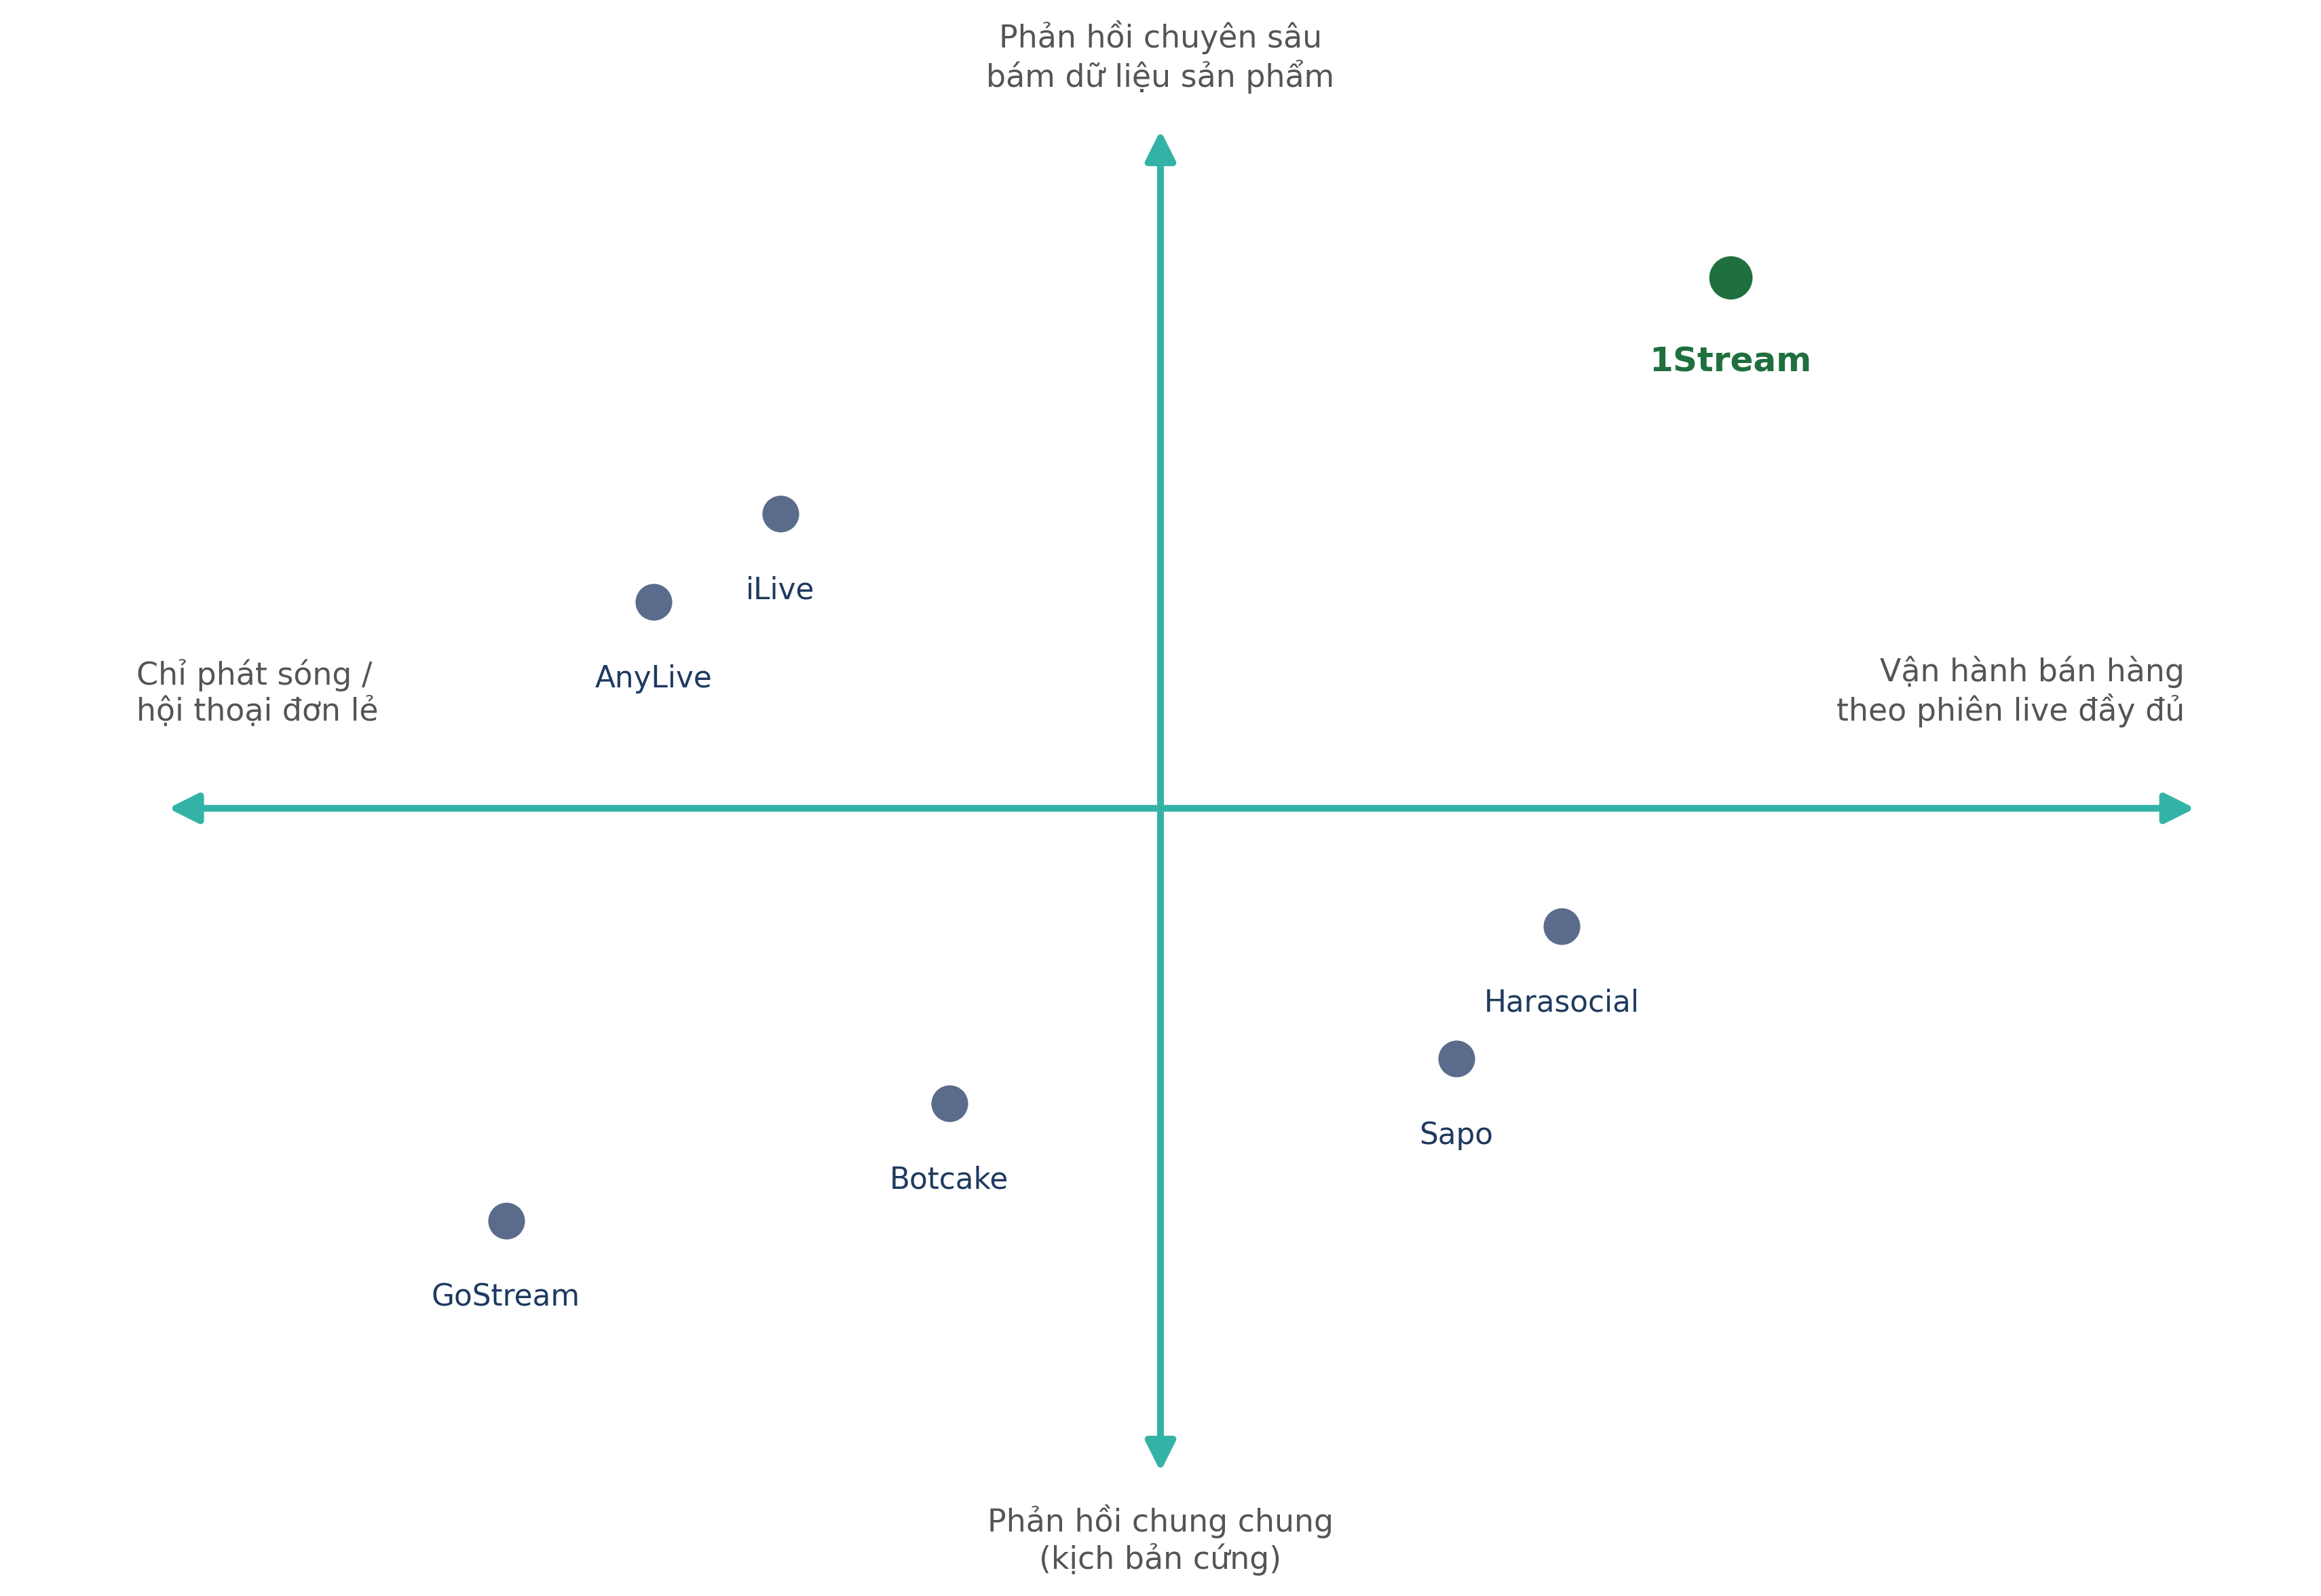
\includegraphics[width=\textwidth]{imgs/positioning_map.png}
    \caption{Bản đồ định vị cạnh tranh của 1Stream so với các giải pháp hiện có}
    \label{fig:positioning-map}
\end{figure}

Bản đồ định vị được xây trên hai trục. Trục ngang thể hiện mức độ hỗ trợ vận hành
bán hàng theo phiên live (từ ``chỉ phát sóng / hội thoại đơn lẻ'' đến ``vận hành
theo phiên live đầy đủ''); trục dọc thể hiện độ chuyên sâu của phản hồi (từ
``kịch bản cứng, chung chung'' đến ``chuyên sâu, bám dữ liệu sản phẩm''). Bốn góc
phần tư cho thấy rõ các nhóm đối thủ đang đứng ở đâu:

\begin{itemize}
    \item \textbf{Góc trên trái (chuyên sâu nhưng thiên nội dung):} iLive và
    AnyLive mạnh về tạo host ảo và nội dung bằng A.I, nhưng chưa đi sâu vào vận
    hành cả một phiên bán hàng theo dữ liệu sản phẩm của từng shop.
    \item \textbf{Góc dưới phải (vận hành mạnh nhưng phản hồi chưa chuyên sâu):}
    Harasocial và Sapo rất tốt ở chốt đơn và quản lý bán hàng đa kênh, song phản
    hồi chủ yếu phục vụ chốt đơn, chưa tối ưu cho tư vấn bám ngữ cảnh sản phẩm
    đang live.
    \item \textbf{Góc dưới trái (đơn giản, phản hồi cơ bản):} GoStream chỉ giải
    quyết khâu phát sóng; Botcake là chatbot theo kịch bản. Cả hai nhẹ và rẻ
    nhưng không chuyên sâu cho livestream bán hàng.
    \item \textbf{Góc trên phải (khoảng trống mục tiêu):} hiện gần như chưa có
    đối thủ nào phủ đồng thời hai yếu tố ``vận hành theo phiên live đầy đủ'' và
    ``phản hồi chuyên sâu bám dữ liệu sản phẩm''. Đây chính là vị trí \textbf{1Stream}
    lựa chọn.
\end{itemize}

Vị trí trên bản đồ cho thấy 1Stream không cạnh tranh trực diện với thế mạnh sẵn
có của từng nhóm (host ảo của iLive, chốt đơn của Harasocial, giá rẻ của
GoStream), mà chọn khoảng trống ở góc trên--phải: một quy trình vận hành
livestream chuyên sâu, bám dữ liệu sản phẩm, chi phí hợp lý và dành riêng cho
shop nhỏ/SME. Nói cách khác, 1Stream không định vị là giải pháp ``đầu tiên'' hay
``duy nhất'', mà nằm ở khoảng giao của ba nhóm --- AI livestream, chatbot bán
hàng và phần mềm vận hành livestream. Lợi thế bền vững của sản phẩm không nằm ở
từng tính năng đơn lẻ (avatar, chatbot, auto-reply hay phát đa nền tảng đều đã
có), mà ở dữ liệu vận hành tích lũy theo ngành hàng, cách chuẩn hóa knowledge
base của từng shop và nguyên tắc phân luồng giữa rule-based logic, AI Agent và
người bán thật.